\documentclass[thesis.tex]{subfiles}

\section{Theoretical Overview}
\subsection{Machine Learning}

\subsection{Neural Networks \& Deep Learning}

\subsection{Object Detection With Convolutional Neural Networks}

\subsection{Computational Graphs}
Although they are commonly visualized as layers of neurons, neural networks are more often represented as computational graphs.

Computational graphs are directed graphs that express a series of computations. Each node is either an input variable, or, when there are incoming edges, a function of those edges' tail nodes. Edges simply denote dependencies between nodes (eg. $a = b + c$).

\begin{figure}[htp]
	\centering
	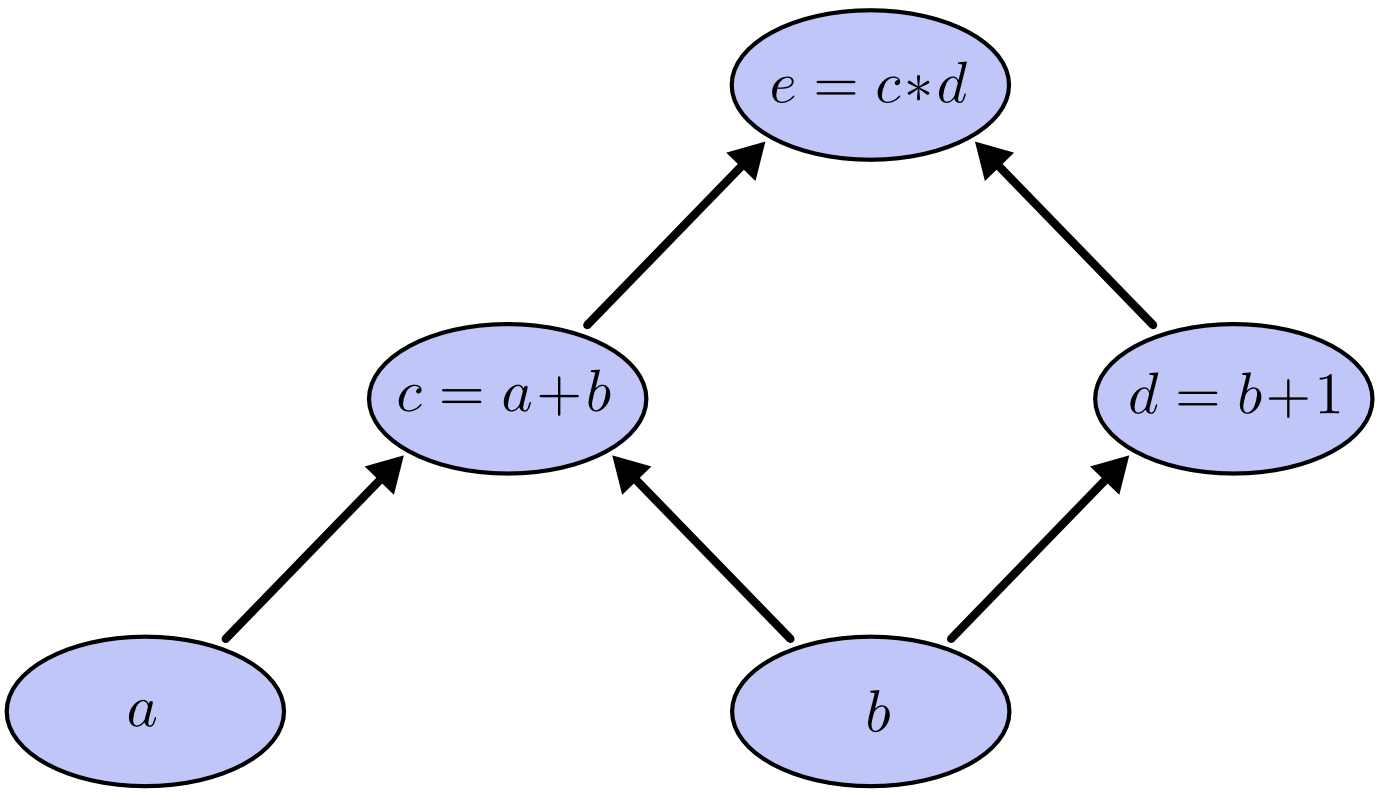
\includegraphics[width=0.5\textwidth]{cgraph1.png}
	\caption{An example computational graph with inputs $a$, $b$ and outputs $(a + b)(b + 1)$}
	\label{fig:cgraph1}
\end{figure}

It is trivial to traverse the graph from all input nodes to calculate its outputs. If we model a neural network as a series of computations (eg. $y = sigmoid(x \cdot w)$), then this corresponds to the network's forward pass. Conversely, since each node knows about its outcoming edges and operator, it can infer the gradient w.r.t each edge. In other words, we can calculate gradients at each node automatically, by traversing the graph backwards. This is immensely helpful for backpropagation, which requires the gradient for each neuron to be calculated.

\begin{figure}[htp]
	\centering
	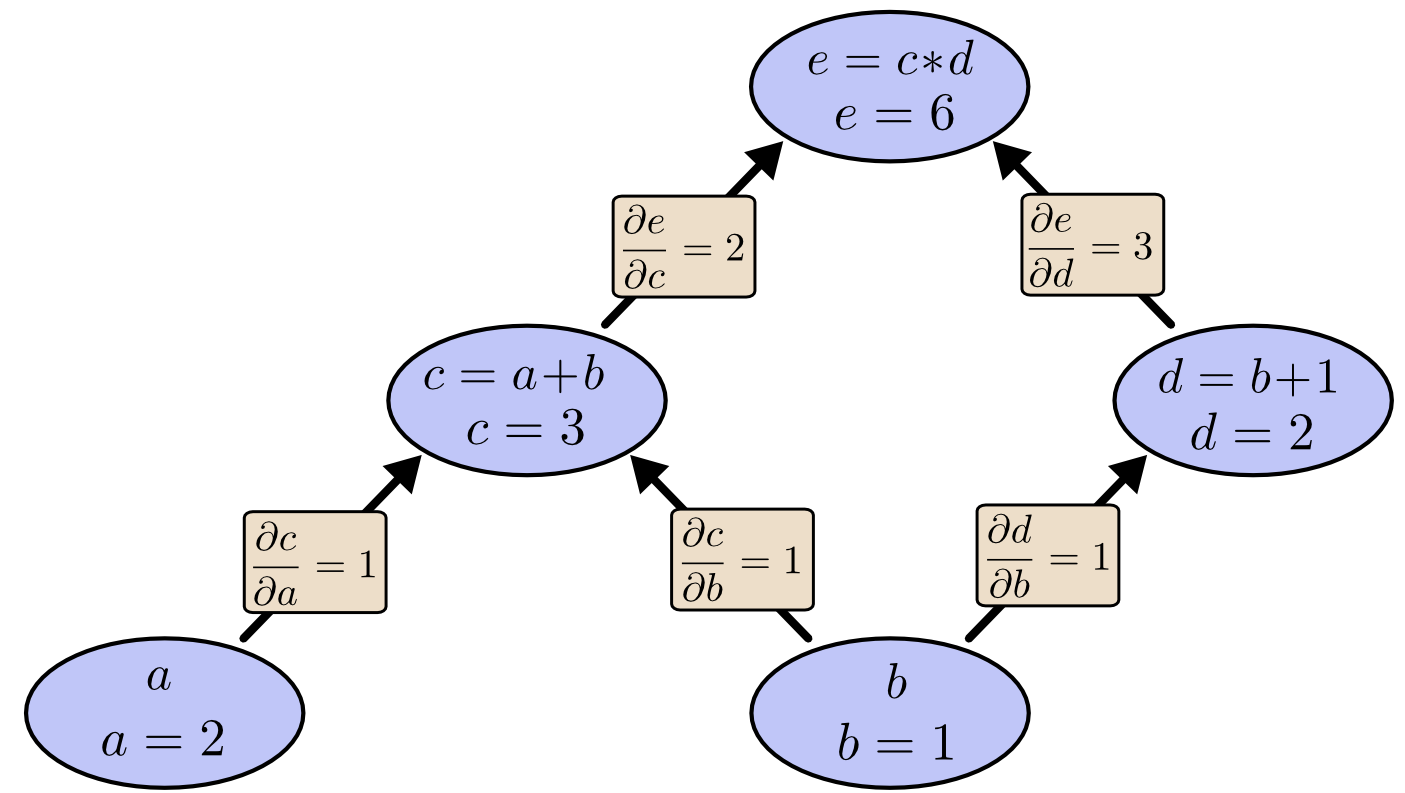
\includegraphics[width=0.5\textwidth]{cgraph2.png}
	\caption{Calculating gradients on each edge}
	\label{fig:cgraph2}
\end{figure}

The fact that neural networks can be modeled as computational graphs has several implications.

\subsection{Training Neural Networks in Parallel}
A major drawback for deep neural networks is the computational complexity of training them. LeNet (1998) \cite{lecun1998lenet}, for example, has over 100,000 parameters, while ResNet-50 (2016) \cite{he2016resnet} has 25 million. Optimizing these parameters over many iterations is very computationally intensive, and training even a small network such as LeNet could take several days on standard CPUs.

A breakthrough for training DNNs was the use of Graphic Processing Units (GPUs), as first presented by Raina et al \cite{raina2009gpu}in 2009. Similar to graphics processing, neural networks are trained using operations on large matrices, which benefit from GPUs' multi-core design. Since then, the toolchain for GPU-accelerated neural network has matured significantly. Libraries such as CUDA, CUDNN \cite{chetlur2014cudnn}, and high level interfaces have made training of neural networks on GPUs trivial.

While GPUs have greatly improved DNN training speed, modern networks continue to be even more complex, along with larger training datasets. This requires more scalable training mechanisms, particularly on multiple devices. One approach, as seen with Google's Tensor Processing Units (TPUs) \cite{jouppi2017datacenter}, is building custom hardware that are designed to work as clusters. Indeed, TPUs are very efficient and performant. However, this approach is often expensive and requires a lot of effort for deployment. A more compact, user-friendly approach is to make use of existing GPUs and computer architectures. This can be done using a software layer that handles communication between GPUs/CPUs on different machines.

Any attempt to train DNNs in a distributed manner is a challenge in maintaining consistency. Even though both the forward and backward pass of a neural network can be effortlessly parallelized (by simply splitting the batch dimension), parameters need to be updated consistently on every node.

\subsection{Deep Learning Frameworks}
